\section{Research Questions}
\label{section-research-questions}
%%%%%%%%%% Isabel Evans suggests adding a table with my RQs at the start of this section. TBD. COULD-DO. Certainly it seems this section needs polish.

%MUST-DO \yijun{If possible, you may need to dig out a few MobileSoft research papers to give evidence that these research questions have not been addressed in literature, e.g., \emph{Future Trends in Software Engineering Research for Mobile Apps}~\sidecite{nagappan2016_future_trends_in_sw_eng_for_mobile_apps}, whether the future work of some paper suggests one does not know the sources, value, or impact of mobile analytics to assess and improve app quality? Is there nothing in the general SE literature studying the "analytics" to "general software quality" problem? If there are such general work, how does "mobile analytics" and "app quality" differentiate the RQs to existing ones...}


My research hypothesis is that using mobile analytics can help improve both the work development teams do and the quality of the products they create. Here work includes the development, testing, and bug investigation of the software being created. For the quality of the product, this research is focusing on a subset of qualities which are \gls{glossary-technology-facing}, %technology-centric, 
and in particular the \gls{glossary-reliability} and \gls{glossary-stability} of the mobile apps when they are in use.

The core question the research aims to consider is:

\begin{quote}
  \emph{How can applying mobile analytics improve the reliability of mobile apps and software development for mobile apps in practice?}~\label{overall-research-question}\index{Research questions}\sidenote{Alternative rewording: "How can applying mobile analytics in software development practice improve the reliability of mobile apps?"}
\end{quote}
% Thanks to https://tex.stackexchange.com/questions/35933/indenting-a-whole-paragraph

\begin{kaobox}
So, you are building on prior work on software analytics for mobile apps but focussing on its practical application by software development teams to improve app reliability. This is important because app reliability, as measured by crash rates and ANRs is key metric in the mobile app eco system. Because this metric is used by the platform provider to determine whether an app should be given access to the ecosystem, it is something developers should pay attention to. In order to understand the effect of applying mobile analytics on the software development practices for  improving reliability of apps, we need to explore the processes, artefacts and tools associated with these activities. This research investigates these three dimensions based on case studies of different mobile app projects, to identify both the current practices and opportunities for improvement provided by using mobile analytics.
\end{kaobox}

To expand on the research question:
\begin{itemize}
    \item \textbf{Applying mobile analytics}: is the use of mobile analytics in order to effect improvements to the practices and the artefacts. Applying mobile analytics refers to both collecting data from the usage of the app and also making use of the analysis of this data to identify and address issues that can improve the app. Improvement of the app focuses on increasing the stability/reliability by reducing ANRs, crashes, and through improving how the app handles various errors (typically reported through Exceptions~\footnote{Exceptions are a core construct in Java programs intended to make those programs robust~\cite{robillard2000_designing_robust_java_programs_with_exceptions}, and similarly \glspl{glossary-exception} are core to Android apps}).
    \item \textbf{Mobile analytics}: Analytics where the data is collected by software running on mobile smartphone-based devices pertaining to the app's qualities-in-use. This research focused on analytics collected pertaining to the stability of the app, where stability includes the reliability of the app.
    \item Software development: includes tasks performed by the software developers including design, coding, testing, bug reporting, and bug tracking.  Use of Scrum development practices, following recommendations and guides that include application compatibility, \gls{ui} guidelines, and designing for performance and responsiveness, \emph{etc}. [Software] testing~\sidecite[][pp.398 - 399]{wasserman2010_software_engineering_issues_for_mobile_app_devt}.~\sidenote{This short paper skims over topics without evidence developers actually do them. Their survey, cited in this paper isn't available so appears to have not actually been published.}
    \item Reliability and Stability are two intertwined measures of software quality in use. There are contradictory opinions on their relationships to each other and to their contributions to software quality, these will be discussed in Chapter~\secref{chapter-related-work}. 
    \item In practice: the key scope of measurement focuses on the efficacy in real-world projects from the perspective of software practitioners who develop mobile applications.
\end{itemize}

In order to answer this research question it is appropriate to consider improvements to the \emph{app i.e. the product} and to the \emph{processes/practices} development teams apply when they develop and maintain their mobile apps. Improvements cannot be be usefully considered in isolation, they need to be grounded in the current practices: the developers will have their perspectives on their use of mobile analytics, and their development artefacts may provide cross-verification of what they say they do compared with tangible evidence of how they use those mobile analytics tools. 

Furthermore, there may be constraints and/or limitations in the current mobile analytics tools which may adversely affect the improvements development teams are able to make to their processes/practices and to their products, hence it is also germane to consider improvements to the current mobile analytics tools.

These additional supporting questions can be restated as six distinct yet related perspectives.

\begin{figure*}
    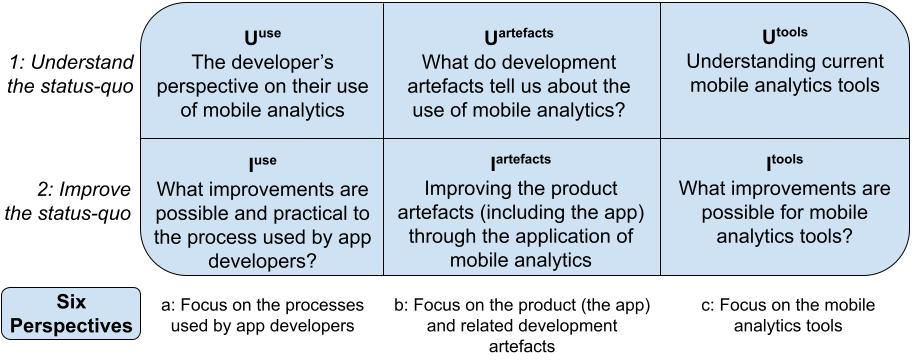
\includegraphics[width=\linewidth]{images/my/six-perspectives-2x3-matrix-12-nov-2021.jpeg}
    \caption{Six Perspectives of Mobile Analytics}
    \label{fig:six-perspectives-in-the-research-questions-section}
\end{figure*}

\subsection{Research questions lead to six perspectives}~\label{rq-leads-to-six-perspectives}
The six perspectives are illustrated in Figure~\ref{fig:six-perspectives-in-the-research-questions-section}~\sidenote{Source figure:~\href{https://docs.google.com/drawings/d/1SafKu3uqgl-s8-I8iWSSWmFY4NdlNpw8v6ZiJDGh50c/edit?usp=sharing}{Google Docs: Six Perspectives drawing}.} and paraphrased below:

\begin{enumerate}
    %\setlength\itemsep{-0.5em} %\itemsep0em
    \item [1a] What do app developers say they do in terms of using mobile analytics? (understand the \emph{status quo} from their perspective).\index{Research questions}
    \item [2a] What's possible in terms of improving their processes, their practices through using mobile analytics?)
    \item [1b] What does their source code (and other available development artefacts) tell us about their use of mobile analytics? (\emph{i.e.} to understand current behaviours in terms of the code that's implemented.
    \item [2b] What's possible in terms of improving the product (and particularly the mobile app) through the application/use of mobile analytics?
    \item [1c] What do we learn about various current mobile analytics tools?
    \item [2c] What improvements are possible for mobile analytics tools based on what was learned in the various case studies?
\end{enumerate}

These provide clear grouping for each of the three columns: on processes (a), on apps and related development artefacts (b), and on the analytics tools (c) which are considered in terms of first understanding and then improving the \emph{status-quo}, shown as two rows, \emph{i.e.} a 3x2 matrix. 


% https://www.skmurphy.com/blog/2014/01/27/difference-between-a-hypothesis-and-an-assumption/
Here the hypothesis is that analytics can help, as stated by Buse and Zimmermann ~(\citeyear{buse_analytics_2010}); and \emph{``with explicit and implicit feedback now available (almost) continuously, questions arise. How can practitioners use this information and integrate it into their development processes [to decide when to release updates]?"}~\sidecite{maalej2016_towards_data_driven_requirements_engineering}.


\section{Research contributions}
Before this research little was known about developers integrating mobile analytics into their artefacts and/or their processes. Unknown were - how, why, and when, they used the outputs of the mobile analytics. Furthermore, little was known about the mobile analytics tools and services used by app developers in industry or in real-world mobile apps.

\newthought{Other forms of software analytics}: 
Software analytics was a recently established field of research - Microsoft used usage data to measure and improve Windows Software. A longitudinal study using custom opensource mobile analytics, called Insight, demonstrated ways in-app mobile analytics was able to help developers of two popular apps to improve the performance of their mobile apps.

Ratings and reviews provided information about problems and failures in mobile apps.

\subsection{My contributions to knowledge}:
The research contributes to the understanding of tools and information seldom available to research - of professional app developers, their artefacts, and of professional mobile analytics tools and services. 

\newthought{Processes}: 
My research contributes knowledge on the approaches various app development teams apply when they use mobile analytics including the selection, integration of code and services, and their application of mobile analytics to detect, identify, and address errors and failures reported by mobile analytics. It builds on prior research, for example, on Insight, and confirms their findings. It contributes new knowledge in the adoption platform-level and commercial in-app mobile analytics, including a) usage patterns by development teams ranging from individual  developers, small teams and large,  \gls{glossary-sharded}\sidenote{\href{https://en.wikipedia.org/wiki/Shard\_(database\_architecture)}{Wikipedia: Shard (database architecture)}} teams, and b) public opensource projects, hybrid projects that combined private and proprietary practices, through to a development team at a major corporation.

Some of the findings were surprising in terms of the patterns of use and in the efficacy of using mobile analytics to achieve significant improvements.

Development teams who embedded mobile analytics into their ongoing, core practices, were able to achieve highly reliable and stable apps. 

\newthought{Artefacts}: 
The research extended prior art in studies of opensource mobile app codebases, with a focus on the use of the most popular product offering: Firebase Analytics. Developers often incorporated multiple mobile analytics libraries into a single mobile app, each for a specific purpose. When developers addressed failures reported by mobile analytics they often modified the source code of the app; these modifications were generally small, yet the effects on improving the reliability/stability of the app were material. 

It also contributes insights from proprietary, commercial codebases and issue tracking artefacts where development teams intermittently filed bug reports for issues reported by mobile analytics.

\newthought{[Mobile  Analytics] Tools}:
The research identified characteristics of a wide range of mobile analytics tools that serve Android app developers in particular. It also found and  presents a range of flaws found in professionally-developed mobile analytics tools, including several of the most-used mobile analytics offerings.

The research contributes material relevant to professional app developers and to the developers of mobile analytics. 

Improvements were identified in all three areas and some of these were implemented during the research. 

Note: In addition to specifying my research contributions add explicit summaries of my contributions that have already been published.

\subsection{Practical impact of my work}
Several of the tool development organisations including Amplitude, Google, and Iteratively actively sought insights and updates from my research. They improved various aspects of their respective mobile analytics offering.

App developers who applied the techniques described in my research were consistently able to significantly improve the reliability/stability of their apps.
